\documentclass[margin = 2cm]{article}

\usepackage{polski}
\usepackage{graphicx}
\usepackage{listings} %listingi kodu
\usepackage{array}
\usepackage{float}
\usepackage{amsmath}
\usepackage{multicol} %kolumny
\usepackage[margin=0.8in]{geometry}
\usepackage{gensymb} %stopnie (symbol)

\graphicspath{ {./images/} } %obrazy

\begin{document} %tytuł
\title{\textbf{Sprawozdanie z laboratorium \\Systemy i sieci przemysłowe}} % \\ robi nową linię
\author{Maciej Misiewicz\\215305 \and Oskar Zieliński\\215373 \and Dariusz Witek vel Witkowski\\215364 \and Szymon Panek\\215319}

\maketitle


\newpage
\tableofcontents
\newpage

%%%%%%%%%%%%%%%%%%%%%%%%%%%%%%%%%%%%%%%%%%%%%%%%%%%%%%%%%%%%%%%

\section{Ćwiczenie 1: Komunikacja CAN}
	\subsection{Cel ćwiczenia}
	Celem ćwiczenia było zapoznanie się z komunikacją za pomocą protokołu CAN na przykładzie połączenia z częścią składową robota hipermobilnego Wheeeler. Ćwiczenie obejmowało wysyłanie rozkazów oraz odbieranie informacji od lokalnego sterownika za pomocą ramek danych.
	\subsection{Realizacja ćwiczenia}
	\subsubsection{Konfiguracja połączenia z robotem}
	Konfiguracja połączenia z robotem ograniczała się do określenia dwóch parametrów - prędkości transmisji jako 1Mbit/s oraz formatu identyfikatora jako format extended.
	\begin{figure}[H]
		\centering
		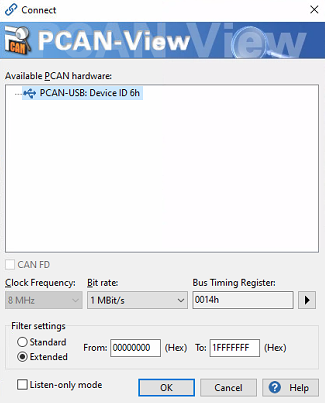
\includegraphics[width=0.5\textwidth]{0}
		\caption{Okno nawiązywania połączenia}
	\end{figure}
	Po udanym połączeniu zostały odebrane trzy ramki danych.
	\begin{figure}[H]
		\centering
		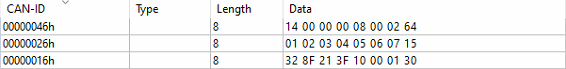
\includegraphics[width=0.9\textwidth]{0_1}
		\caption{Odebrane ramki danych}
	\end{figure}
	\begin{figure}[H]
		\centering
		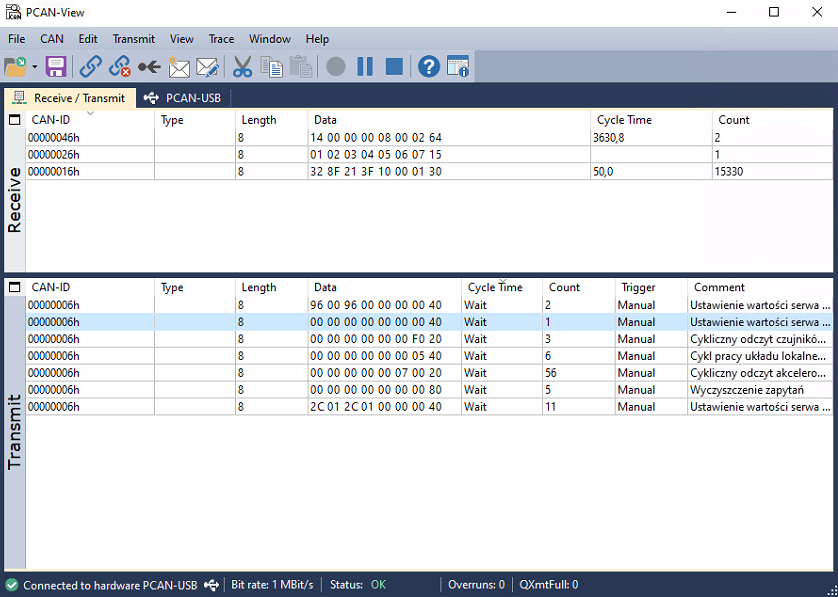
\includegraphics[width=0.9\textwidth]{interfejs}
		\caption{Widok interfejsu w programie PCANView}
	\end{figure}
	\begin{figure}[H]
		\centering
		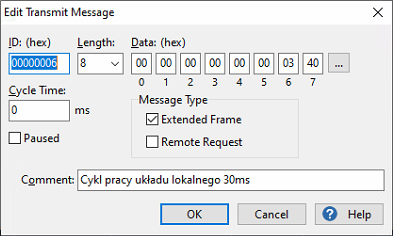
\includegraphics[width=0.6\textwidth]{edytorinstrukcji}
		\caption{Kreator rozkazów}
	\end{figure}
	\subsubsection{Ustawienie cyklu pracy układu lokalnego 30ms}
	\label{a}
	Ustawienie cyklu pracy układu lokalnego odbywa się za pomocą 6 bajtu, podana w nim wartość w zakresie 2-20 (dec) zwiększających cykl co 10ms. Bajt 7 odpowiada za ustawienie zadanych wartości w instrukcji.  Ramka realizujaca zadanie wygląda następująco:
	
	00000006h	00 00 00 00 00 00 03 40
	
	\begin{figure}[H]
		\centering
		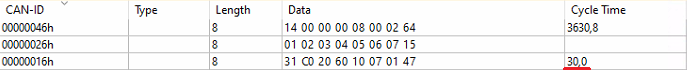
\includegraphics[width=0.9\textwidth]{30ms}
	\end{figure}
	
	\subsubsection{Ustawienie cyklicznego odczytu danych z akcelerometru}
	Ustawienie odczytu danych z akcelerometru odbywa się za pomocą 4 bajtu. Ustawiona wartość 07 jest składową odczytu osi X, Y i Z. Bajt 7 odpowiada za cykliczne odczytywanie pomiarów. Ramka realizujaca zadanie wygląda następująco:
	
	00000006h	00 00 00 00 00 07 00 20
	\subsubsection{Ustawienie cyklicznego odczytu danych z czujników odległości}
	Ustawienie odczytu danych z czujników odległości odbywa się za pomocą 6 bajtu. Ustawiona wartość F0 jest składową adresów 4 czujników odległości. Bajt 7 odpowiada za cykliczne odczytywanie pomiarów. 
	
	00000006h	00 00 00 00 00 00 F0 20
	\subsubsection{Zmiana położenie serwa 1 i serwa 2}
	Zakres roboczy obu serw mieści się między 0 a 300 (dec), naszym zadaniem było ustawienie 3 zadanych pozycji: minimalnej, środkowej oraz maksymalnej. Wysterowanie pojedynczego serwa odbywa się przy pomocy dwóch bajtów. Dla serwa 1 jest to bajt0 oraz bajt1, natomiast dla    serwa 2  bajt2 oraz bajt3.
	

	\begin{itemize}
	\item Maksymalna pozycja serw:
	
	00000006h	2C 01 2C 01 00 00 00 40
	\begin{figure}[H]
		\centering
		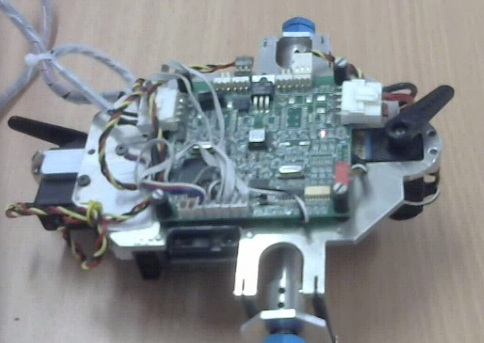
\includegraphics[width=0.6\textwidth]{max}
	\end{figure}
	 \item Środkowa pozycja serw:
	
	00000006h	96 00 96 00 00 00 00 40
	\begin{figure}[H]
		\centering
		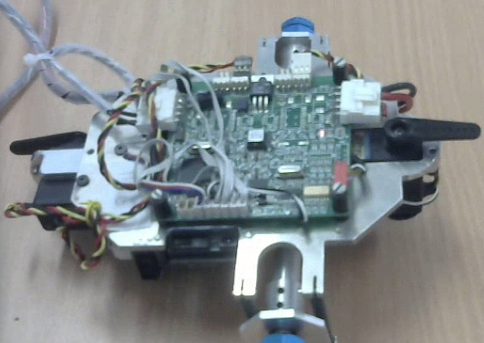
\includegraphics[width=0.6\textwidth]{middle}
	\end{figure}
	\item Minimalna pozycja serw:
	
	00000006h	00 00 00 00 00 00 00 40
	\begin{figure}[H]
		\centering
		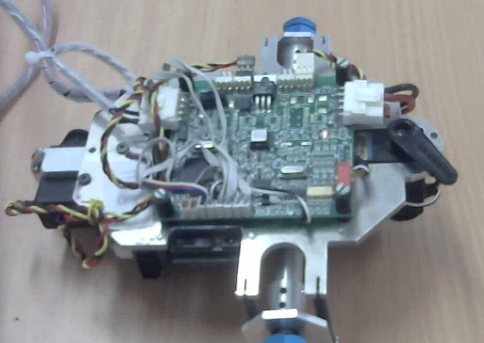
\includegraphics[width=0.6\textwidth]{min}
	\end{figure}

	\end{itemize}
	\subsubsection{Zmiana cyklu pracy układu lokalnego na 50ms}
	Analogicznie do punktu \ref{a}, zmianie uległa jedynie zadana długość cyklu.
	
	00000006h	00 00 00 00 00 00 05 40
	\begin{figure}[H]
		\centering
		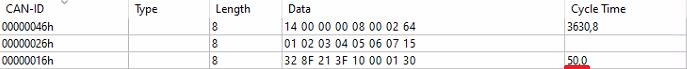
\includegraphics[width=0.9\textwidth]{50ms}
	\end{figure}
	\subsection{Wnioski i spostrzeżenia}
	Oprogramowanie PCANView jest łatwym, czytelnym i intuicyjnym narzędziem. Bezpośrednio pokazuje komunikację za pomocą ramek, dzieląc je na przychodzące i wysyłane. Jest dobrym programem do testowania oraz podglądu transmisji protokołem CAN. Zaletą jest także możliwość wyboru sposobu wysyłania rozkazów - możemy wysłać ramkę pojedynczo manualnie lub wysyłać cyklicznie w zadanym interwale. Program sygnalizuje status połączenia w protokole. 

%%%%%%%%%%%%%%%%%%%%%%%%%%%%%%%%%%%%%%%%%%%%%%%%%%%%%%%%%%%%

\section{Ćwiczenie 2: Sterowanie manipulatorem za pomocą sterownika CompactRIO (NI)}
	\subsection{Cel ćwiczenia}
Zapoznanie się z ze strukturą FPGA i Real-Time sterownika CompactRIO jego współpracą z środowiskiem programowym LabVIEW na przykładzie sterowania manipulatorem o trzech stopniach swobody.
	\subsection{Realizacja ćwiczenia}
  		\subsubsection{Uzupełnienie brakującej części kodu}
Uzupełnienie brakującej części programu polegało na dodaniu suwaków zadających pozycję poszczególnych złączy manipulatora, których skala została odpowiednio dobrana do zakresu pracy złącz. Dane odbierane z dodanych elementów interfejsu zostają przesłane do bloku FPGA oraz udostępniane jako zmienne globalne środowiska RIO. W celu warunkowego umożliwienia kontroli z poziomu panelu HMI, kod odpowiedzialny za uaktualnianie wartości położenia został objęty blockiem case-if.
	\begin{figure}[H]
		\centering
		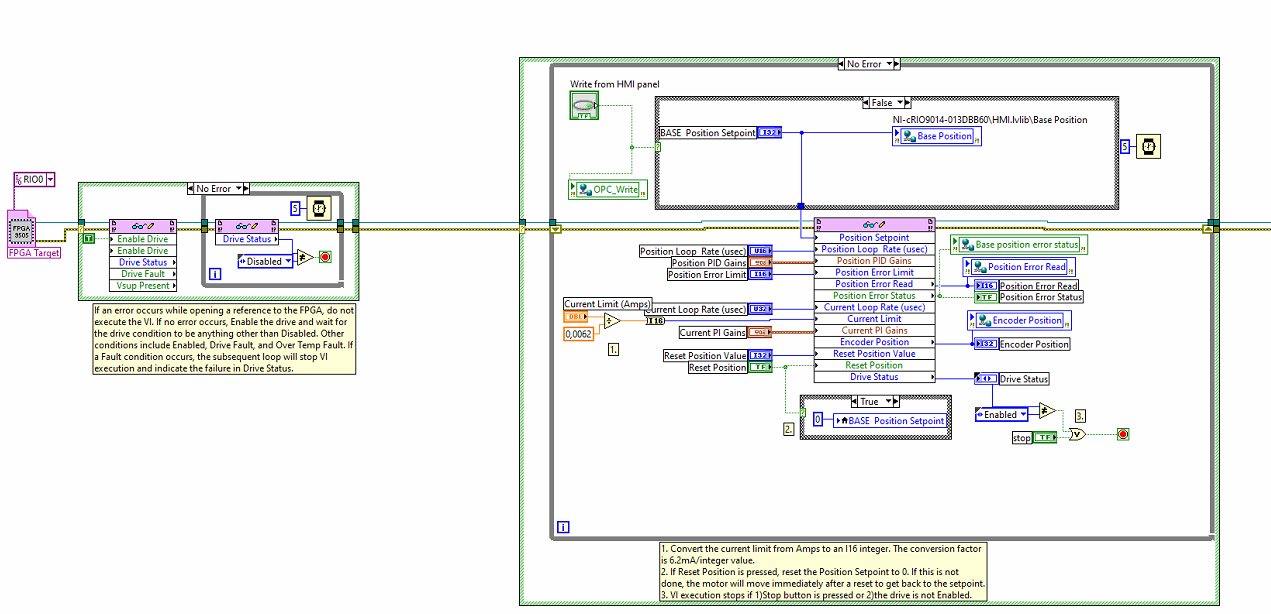
\includegraphics[width=0.9\textwidth]{3_1}
		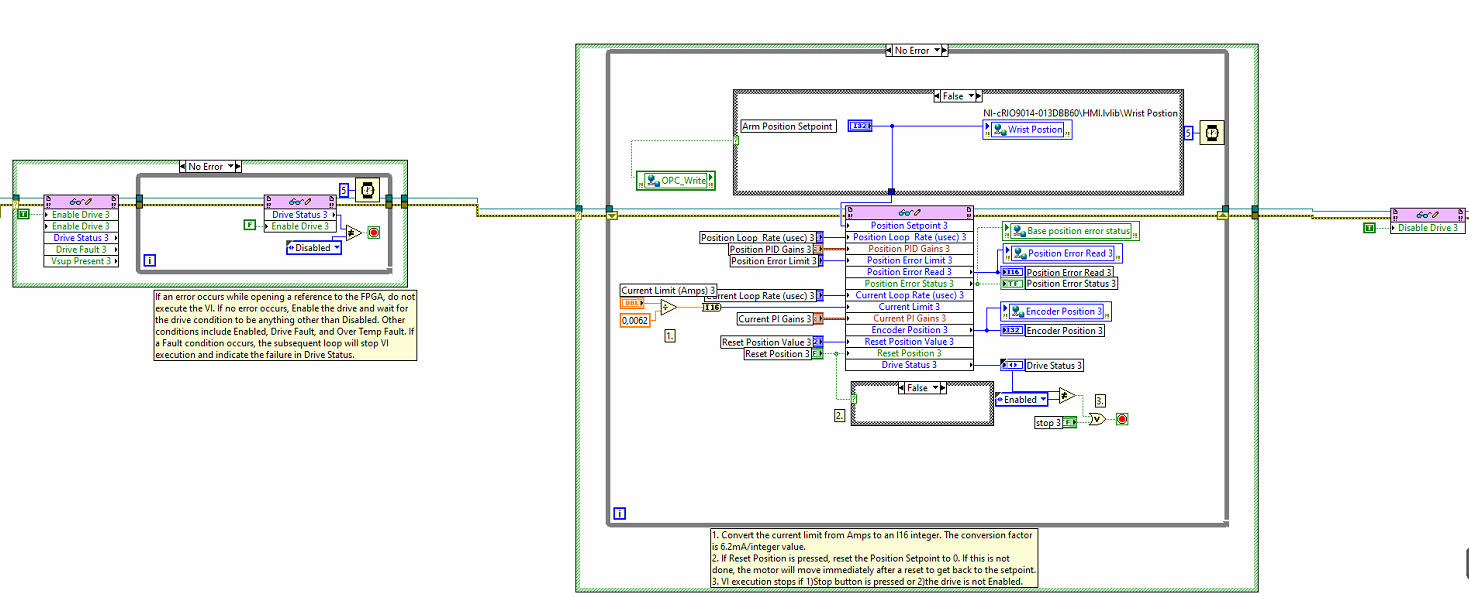
\includegraphics[width=0.9\textwidth]{3_2}
		\caption{Realizacja połączenia panelu kontrolnego użytkownika z blokiem FPGA.}
	\end{figure}

	\begin{figure}[H]
		\centering
		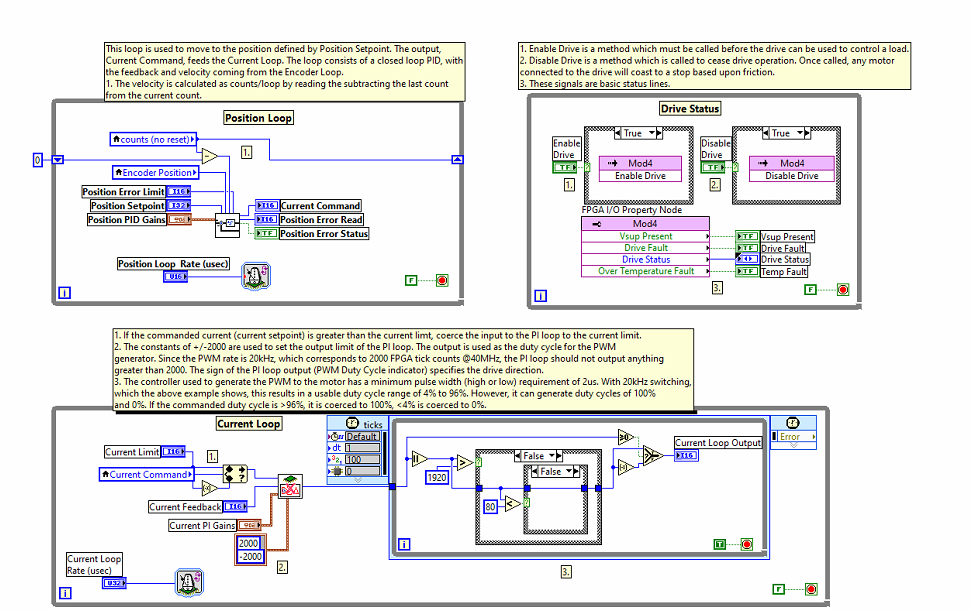
\includegraphics[width=0.9\textwidth]{3_3}
		\caption{Struktura programu FPGA odpowiedzialnego za realizację regulacji pozycji oraz prądu.}
	\end{figure}
	\begin{figure}[H]
		\centering
		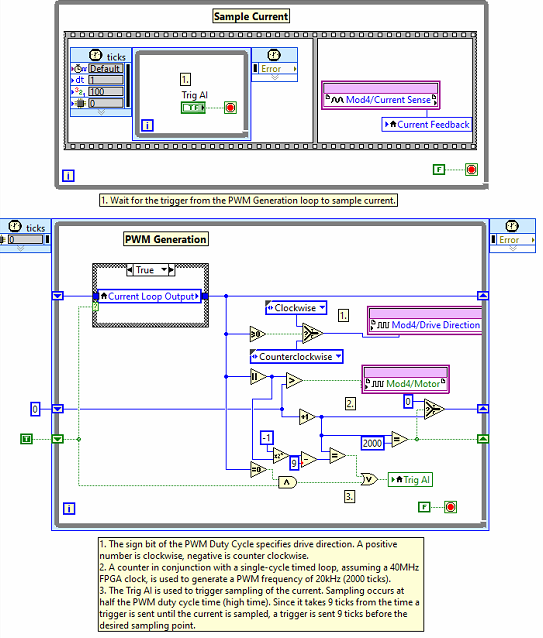
\includegraphics[width=0.5\textwidth]{3_4}
		\caption{Struktura programu FPGA odpowiedzialnego za realizację pomiaru prądu oraz generację sygnału sterującego PWM.}
	\end{figure}
	\begin{figure}[H]
		\centering
		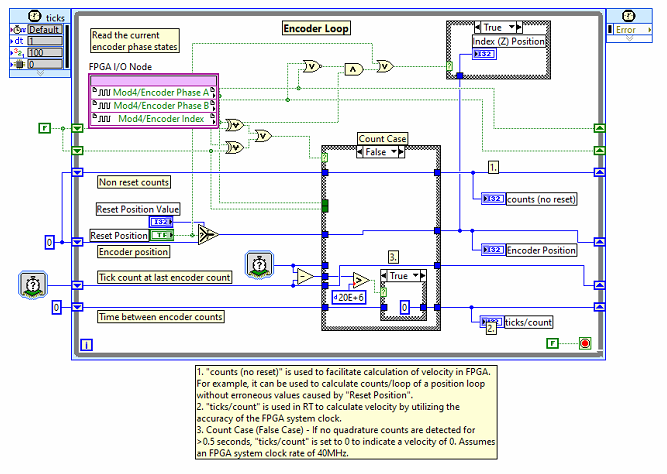
\includegraphics[width=0.7\textwidth]{3_5}
		\caption{Struktura programu FPGA odpowiedzialnego za odczyt oraz interpretację wyjść kanałów A i B enkodera.}
	\end{figure}


		\subsubsection{Dobranie nastaw regulatorów PID dla ramienia oraz nadgarstka robota}

		Po umożliwieniu zadawania pozycji pozostałym złączom, naszym zadaniem było dobranie dla nich nastaw regulatorów. Ograniczyliśmy się do strojenia 				regulatorów pozycji. Nasza metodyka ich doboru opierała się na początkowym zmniejszeniu członu proporcjonalnego Kp tak, aby uzyskać pracę złącz 				pozbawioną oscylacji. Następnie dopiero dobieraliśmy Kp i Kd tak, aby przyśpieszyć proces regulacji, bez ponownego wprowadzenia złącz w stan oscylacji.
		Człon całkujący okazał się niepotrzebny w regulacji pozycji, układ był w stanie osiągnąć wartość zadaną bez znaczącego błędu statycznego.

	\begin{figure}[H]
		\centering
		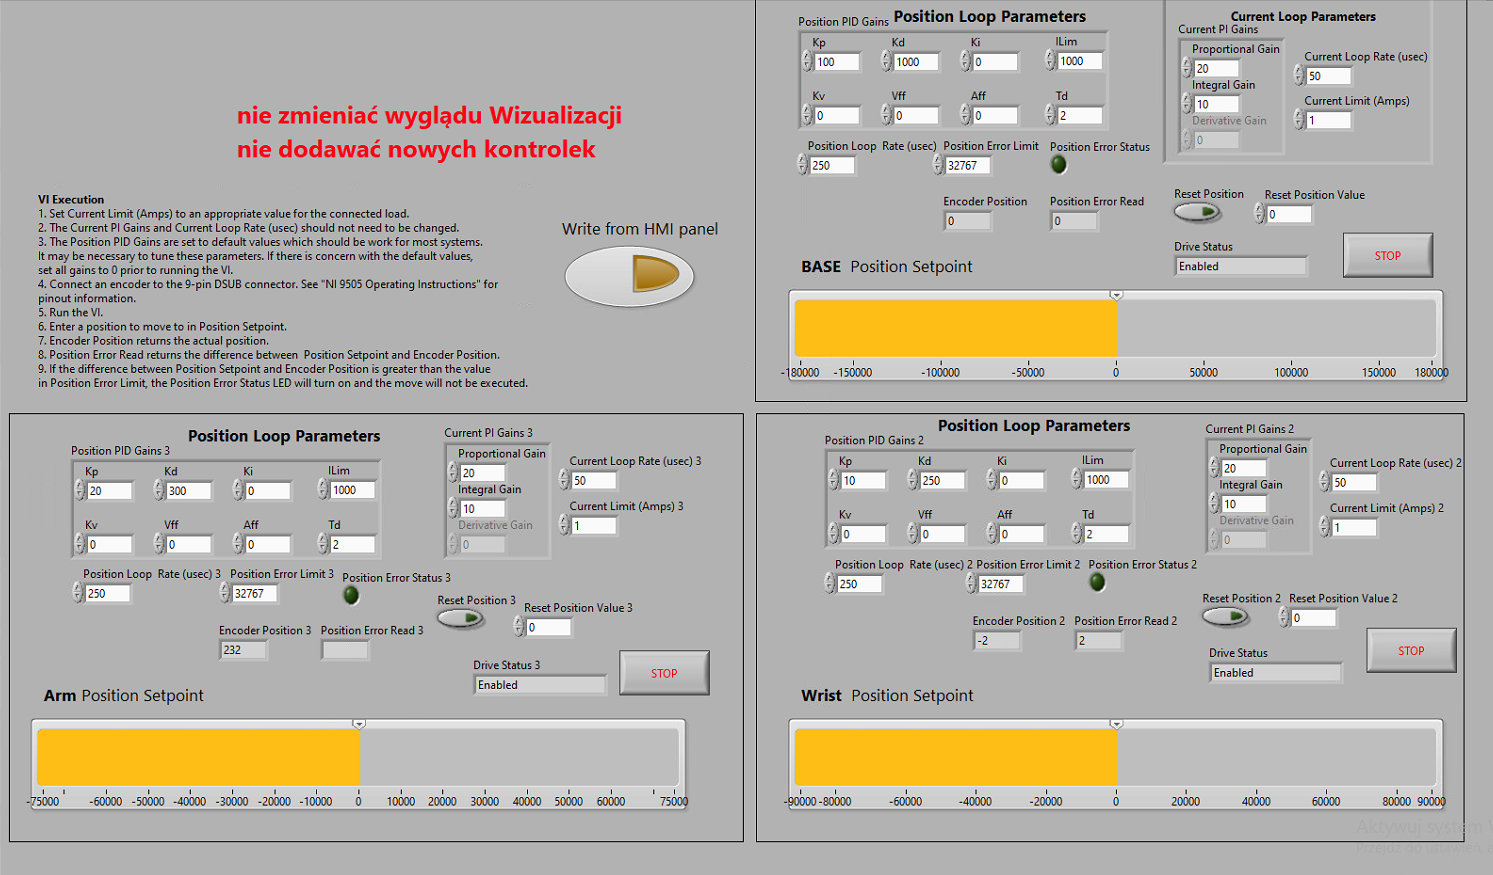
\includegraphics[width=0.9\textwidth]{3_panel}
		\caption{Widok panelu kontrolnego sterowników poszczególnych złącz wraz z dobranymi nastawami regulatorów}
	\end{figure}

	\subsection{Wnioski i spostrzeżenia}
Nastawy regulatorów zostały dobrane w taki sposób, aby ruch poszczególnych złącz manipulatora do pozycji zadanych odbywał się w jak najkrótszym czasie, jednocześnie nie wywołując oscylacji. 

Za szybka zmiana zadanego położenia powodowała gwałtowny skok błędu odczytu enkodera, który był sygnalizowany przez kontrolkę w panelu użytkownika. Błąd ten skutkował zatrzymaniem pracy złącza, czego efektem było niezrealizowanie zadanego położenia.

Podczas realizacji ćwiczenia zauważyliśmy, że zmienne pozycyjne nadgarstka i ramienia są ze sobą zamienione. Może to być spowodowane błędem definicji zmiennych globalnych lub niewłaściwym podłączeniem silników do sterownika.

%%%%%%%%%%%%%%%%%%%%%%%%%%%%%%%%%%%%%%%%%%%%%%%%%%%%%%%%%%%%%%%%%%%

\section{Ćwiczenie 3: Sterowanie robota za pomocą panelu operatorskiego sprzężonego przez sieć
Ethernet ze sterownikiem CompactRIO.}

\subsection{Cel ćwiczenia}

Celem ćwiczenia było zapoznanie się z sterowaniem systemem (w tym wypadku robotem) przy wykorzystaniu dodatkowego urządzenia wyjściowego komunikującego się z sterownikiem za pomocą zmiennych współdzielonych. W trakcie ćwiczenia uzupełnialiśmy kod LabView realizujący funkcjonalność panelu HMI.

\subsection{Realizacja ćwiczenia}

\subsubsection{Kod programu}

\begin{figure}[H]
	\centering
	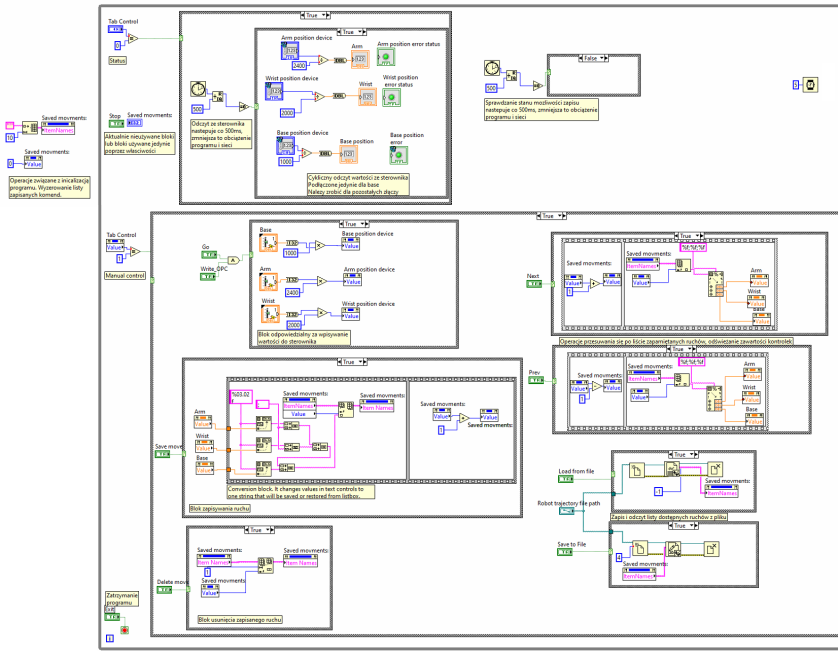
\includegraphics[width=\textwidth]{kod}
	\caption{Diagram pogramu LabView}
\end{figure}

Powyższy diagram implementuje funkcjonalność panelu HMI. Panel operatorski posiada trzy zakładki:

\begin{itemize}
\item Status - węwnątrz tej zakładki wyświetlane były obecne pozycje oraz statusy złącz manipulatora.
\item Manual control - zakładka pozwalała na zadawanie pozycji złącz manipulatora oraz zapisywanie/odczytywanie historii wykonywanych operacji do pliku. 
\item Settings - zakładka pozwalała na wprowadzenie ścieżki pliku zarówno do zapisu jak i odczytu trajektorii.
\end{itemize}

Warto zaznaczyć, że sterowanie ręczne z poziomu 'panelu HMI' było możliwe dopiero po przejściu sterownika w tryb działania manualnego.

W trakcie laboratorium zadaniem naszej grupy było dokończenie dwóch bloków funkcjonalnych diagramu, odpowiedzialnych za zapis oraz odczyt pozycji poszczególnych złącz z sterownika.

\begin{figure}[H]
	\begin{minipage}[t]{0.4\textwidth}
	\centering
	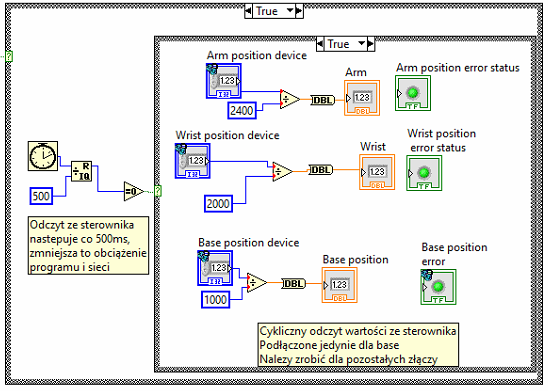
\includegraphics[width=\textwidth]{odczyt}
	\caption{Kod odpowiedzialny za odczyt pozycji złącz manipulatora}
	\end{minipage}
	\hfill
	\begin{minipage}[t]{0.49\textwidth}
	\centering
	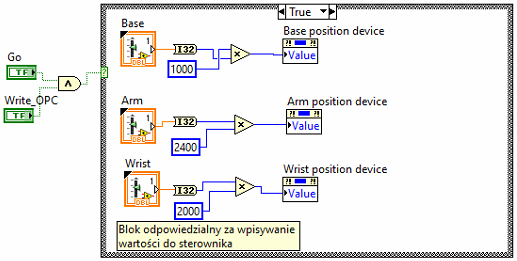
\includegraphics[width=0.94\textwidth]{zapis}
	\caption{Kod odpowiedzialny za zapis pozycji złącz manipulatora}
	\end{minipage}
\end{figure}

W ramach realizacji kodu, musieliśmy dodać dwie brakujące zmienne złączowe Arm oraz Wrist, a także powiązać je  z odpowiednimi zmiennymi współdzielonymi. Musieliśmy również dokonać odpowiedniego przeskalowania wartości zmiennych zarówno wysyłanych do jak i odbieranych od sterownika. Odpowiednie wartości skalujące zostały wyznaczone na podstawie zakresów zmiennych złączowych podanych w instrukcji laboratorium.

\begin{figure}[H]
	\centering
	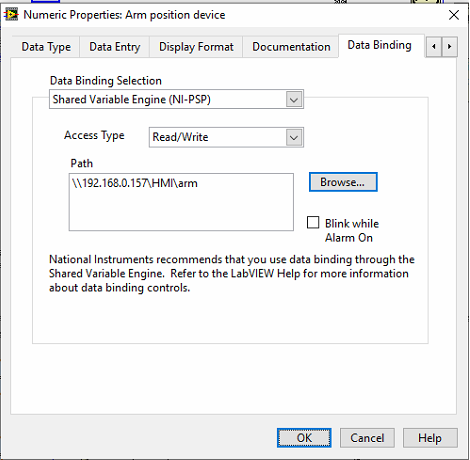
\includegraphics[width=0.5\textwidth]{zmiene}
	\caption{Powiązywanie zmiennych Arm oraz Wrist z odpowiednimi zmiennymi współdzielonymi}
\end{figure}

\subsubsection{Gotowa aplikacja}

Gotowa aplikacja panelu HMI już pozwalała nam na zadawanie pozycji poszczególnym złączom manipulatora. Sprawne były również pozostałe wcześniej opisane funkcjonalności panelu operatorskiego m.in. zapis historii operacji.

\begin{figure}[H]
	\centering
	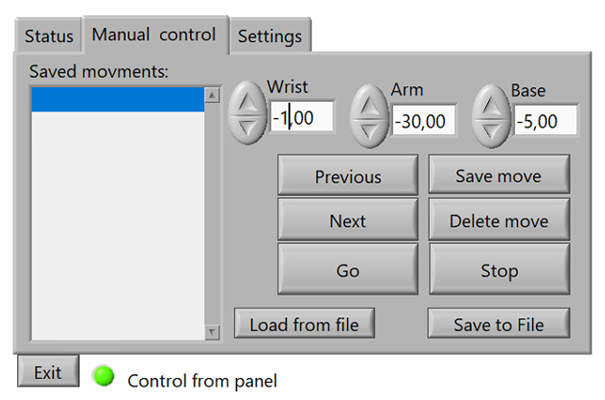
\includegraphics[width=0.65\textwidth]{panel}
	\caption{Widok panelu HMI}
\end{figure}

\begin{figure}[H]
	\centering
	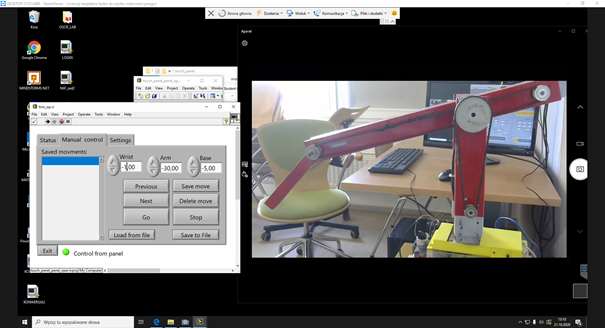
\includegraphics[width=.9\textwidth]{widok}
	\caption{Widok panelu oraz sterowanego robota}
\end{figure}

\subsection{Wnioski i spostrzeżenia}
Komunikacja ze sterownikiem z poziomu panelu operatorskiego funkcjonowała prawidłowo. Nie mieliśmy jednak niestety wpływu na implementacje programu sterownika - w trakcie testów zaobserwowaliśmy, że zmienne złączowe Wrist i Arm były ze sobą zamienione. Przy źle dobranych nastawach regulatorów pozycji poszczególnych złącz, dało się zaobserwować liczne oscylacje przy dochodzeniu do pozycji zadanych. Wnioskujemy również, że w trakcie pracy nad relatywnie dużym projektem programistycznym, działającym  czasem na wielu różnych urządzeniach, przydatne jest ustalenie jednolitej konwencji nazewnictwa zmiennych występujących w projekcie. Zauważyliśmy również, że korzystanie ze zmiennych wspóldzielonych jest prostą w implementacji metodą komunikacji między urządzeniami.



\end{document}